
%%%%%%%%%%%%%%%%%%%%%%%%%%%%%%%%%%%%%%%%%%%%%%%%%%%%%%%%%%%%%%%%%%%%%%%%%%%%%%%%%%
\begin{frame}[fragile]\frametitle{}
\begin{center}
{\Large Fast.ai Setup on Google Colab - Manikanta Yadunanda}
\end{center}

\tiny{(Ref: https://towardsdatascience.com/fast-ai-lesson-1-on-google-colab-free-gpu-d2af89f53604)}
\end{frame}

%%%%%%%%%%%%%%%%%%%%%%%%%%%%%%%%%%%%%%%%%%%%%%%%%%%
\begin{frame}[fragile] \frametitle{What is Google Colab?}

\begin{itemize}
\item Google colab allows ipython notebook to be run on Cloud.
\item You can use GPU, K80(at this moment)as a backend for free for 12 hours at a time.
\item You can upload notebooks using File$\rightarrow$Upload Notebook
\item To enable GPU backend for your notebook. Runtime$\rightarrow$Change runtime type$\rightarrow$Hardware Accelerator$\rightarrow$GPU
\end{itemize}
\end{frame}

%%%%%%%%%%%%%%%%%%%%%%%%%%%%%%%%%%%%%%%%%%%%%%%%%%%
\begin{frame}[fragile] \frametitle{Fast ai setup}
\begin{itemize}
\item Every time you login to Google colab, you get a new VM (Virtual Machine). 
\item You will need to install all non-standard libs every-time.
\item Need to download data as well.
\begin{lstlisting}
!pip install fastai
!pip install opencv-python
!apt update && apt install -y libsm6 libxext6
!pip3 install http://download.pytorch.org/whl/cu80/torch-0.3.0.post4-cp36-cp36m-linux_x86_64.whl 
!pip3 install torchvision
!pip install pathlib
!mkdir data && wget http://files.fast.ai/data/dogscats.zip && unzip dogscats.zip -d data/
\end{lstlisting}
\item Apart from data there are other files at http://files.fast.ai/ like ipython notebooks. You can either copy or run them, else you can type them in Google Colab afresh.
\end{itemize}

\end{frame}

%%%%%%%%%%%%%%%%%%%%%%%%%%%%%%%%%%%%%%%%%%%%%%%%%%%
\begin{frame}[fragile] \frametitle{Fast ai Troubleshooting}
\begin{itemize}
\item If it throws GPU error saying it can't connect, thats due to load (lots of people connecting)
\item Sometimes, the runtime just dies intermittently. There may be many underlying causes for this.
\item The amount of ram available is ~13GB which is too good given it is free.But with large networks like our resnet in lesson 1, there are memory warnings most of the times. 
\end{itemize}

\end{frame}

% %%%%%%%%%%%%%%%%%%%%%%%%%%%%%%%%%%%%%%%%%%%%%%%%%%%
% \begin{frame}[fragile] \frametitle{Big Break-through in Vision}
% \begin{center}
% 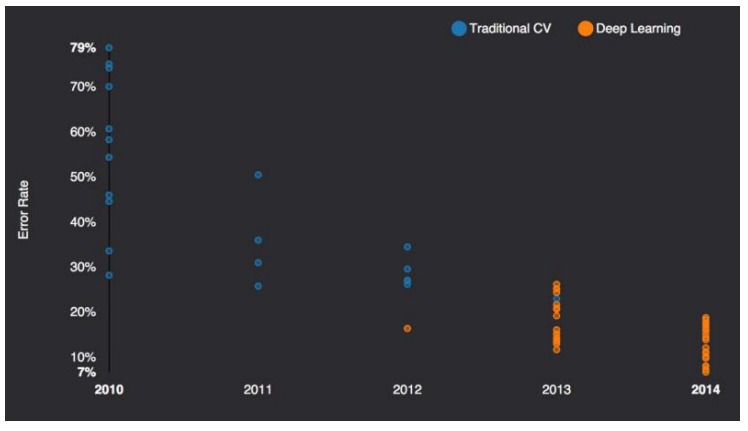
\includegraphics[width=\linewidth,keepaspectratio]{ai38}
% \end{center}
% \tiny{(Reference: Introduction to Deep Learning - Ismini Lourentzou)}
% \end{frame}

%%%%%%%%%%%%%%%%%%%%%%%%%%%%%%%%%%%%%%%%%%%%%%%%%%%%%%%%%%%%%%%%%%%%%%%%%%%%%%%%%%
\begin{frame}[fragile]\frametitle{Other options}
Other than Google Colab
\begin{itemize}
\item You can setup an GPU instance on AWS, as per https://github.com/reshamas/fastai\_deeplearn\_part1/blob/master/tools/aws\_ami\_gpu\_setup.md
\item Similarly video at http://course.fast.ai/lessons/lesson1.html talks about using Crestle and Paperspace cloud services option.
\item To me, Google Colab needs least setup and least money (actually None!!)
\end{itemize}
\end{frame}
